\chapter{相关工作}\label{chap:rel-works}

\section{动力学方程及其离散化}

物理仿真的核心是对于动量PDE的求解:
\begin{equation}
\mathbf F(\mathbf x, t) = M \ddot{\mathbf x}  
\end{equation}
根据物体属性的不同、数学离散化的不同,可以给出该方程的不同离散形式。

% Ref: https://innovationatwork.ieee.org/the-advantages-of-fem/
有限元方法(FEM)是一种用于数值求解工程和数学建模中微分方程的流行方法。它通常用于结构分析、传热、流体流动、质量传输和电磁势等领域。有限元方法有许多优点。例如,它允许更容易地对复杂的几何形状和不规则形状进行建模。有限元方法基于物体的拉格朗日网格表示实现。其将复杂的物体视为简单物体的组合,例如使用三角元、六面体元对于原物体进行剖分,通过计算大量的简单物体的物理量变化,来逼近整个复杂物体的物理量变化。

弹簧质点模型是一种抽象的物理系统,它假设模拟对象要么是质点,要么是弹簧,质点之间通过弹簧连接。经过这样的抽象,要模拟整个系统的物理运动,只需要模拟弹簧质点分别的运动和它们之间的关系即可。弹簧质点模型是对于布料建模的常用手段。

有限体积法(FVM)是一种以数值方法解偏微分方程的计算方式。在有限体积法中,将要描述的物理实体切分为网格单元来描述,并使用散度定理,将所有包含散度项的偏微分方程中的体积积分转换为表面积分。对于流体而言,给定模拟区域,有限体积法将区域进行固定的网格划分,在网格点上存储速度、密度物理量。每一时间步,都根据控制方程的欧拉形式进行解算和更新。

物质点法(MPM)是一种混合拉格朗日/欧拉的PDE求解方法,最近被引入计算机图形学领域。它使用控制方程的连续性描述,并利用用户可控的弹塑性本构模型。MPM允许使用规则的笛卡尔网格来自动的总碰撞和断裂处理。基于MPM原理提出的FLIP算法已经成为流体仿真的经典。

本节将简要介绍 FEM 变形体、弹簧-质点模型布料、MPM方法流体的力学、运动学求解基本原理和算法。本文所考察的物理现象都在三维空间中进行,并在不引起歧义的情况下,不区分各类张量本身与其在标准笛卡尔坐标系下的坐标符号。


\subsection{有限元模型的变形体解算}\label{sec:dyn-solve}

给定几何形体上的 $N$ 个采样点,$\mathbf x_{i}, i = 1\cdots N$,及其剖分得到的单元集合(以四面体为例)$\mathcal T = \{(i, j, k, l)\}$,通过计算采样点的运动,逼近整个几何形体的运动。

图形学中,常用三角元对物体进行剖分,并使用线性基函数对物理量进行插值逼近。运动学模拟求解的是形变函数
$$
\mathcal F: \Omega_0 \rightarrow \Omega_t
$$
其中$\Omega_0$表示初始状态下的物体,$\Omega_t$表示$t$时刻的物体,$\mathcal F$将 $\Omega_0$ 的一点一一地映射到$\Omega_t$上的一点。考虑$t = 0$其上的采样点$\mathbf x_i(0)$,$\mathbf x_i(t) = \mathcal F(\mathbf x_i(0))$。所谓线性基函数是指,对于某个四面体元中$(i, j, k, l)$的任一点 $\mathbf x(0)$,其$t=0$时刻的重心坐标为$(u, v, w)$,则近似其$t$时刻的位置为
$$
\mathbf x(t) = u \mathbf x_j(t) + (1 - u)\mathbf{x}_i(t) + 
 v \mathbf x_k(t) + (1 - v) \mathbf{x}_i(t)
 + w \mathbf x_l(t) + (1 - w) \mathbf{x}_i(t)
$$


\begin{figure}[h!]
  \centering
  \includegraphics[width=0.9\linewidth]{img/Screenshot 2023-04-19 at 10.23.09.png}
  \caption{有限元法空间离散化:将物体离散为四面体,在空间上存储四面体节点的位置与速度,在拓扑上存储节点的四面体连接关系。}
\end{figure}

为描述物体在局部的形变情况,定义物体形变梯度为:
\begin{equation}\label{def:def-grad}
  \mathbf F = \nabla_{\mathbf x} \mathcal F
\end{equation}
对于四面体元$(i, j, k, l)$,利用静止状态和当前状态的位置坐标$\mathbf x_i(0), \mathbf x_i(t)$,计算形变梯度为
\begin{equation}\label{eq:deformation-grad-compute}
\begin{aligned}
  \mathbf F =\mathbf X_{\mathrm{curr}}\mathbf X_{\mathbf{rest}}^{-1} =& [\mathbf x_j(t) - \mathbf x_i(t);\mathbf x_k(t) - \mathbf x_i(t); \mathbf x_l(t) - \mathbf x_i(t)] \\
  &\cdot [\mathbf x_j(0) - \mathbf x_i(0);\mathbf x_k(0) - \mathbf x_i(0); \mathbf x_l(0) - \mathbf x_i(0)]^{-1}
\end{aligned}
\end{equation}

根据线性有限元的基本假设,形变梯度在每一个四面体元$i$中为常量,记为$\mathbf F_i$。在空间中引入笛卡尔坐标系,$\mathbf x \in {\mathbb R}^3, \mathbf F_i \in \mathbb{R} ^{3\times 3}$。矩阵$\mathbf F_i$描述了该四面体元的形变情况。

当前,我们主要考虑超弹性模型。在形变中,超弹性模型保证了弹性能有如下性质:
\begin{enumerate}
  \item 旋转不变性:对于物体的旋转操作不改变弹性能量;
  \item 平移不变性:对于物体的平移操作不改变弹性能量;
\end{enumerate}
其弹性能量密度函数$\Psi$仅依赖于$\mathbf F$。若考虑矩阵 $\mathbf F$的 SVD 分解
\begin{equation}\label{eq:def-grad-svd}
  \mathbf F = U \Sigma V^T
\end{equation}
由于超弹性模型的平移不变性,$\Psi$仅由$\Sigma=\mathrm{diag}(\sigma_1, \sigma_2, \sigma_3)$决定。

常见的超弹性模型有 StVK模型、Neo-Hookean模型等。弹性能量密度函数的不同定义与材料参数 $\lambda, \mu$ 的设置,区分了不同材料的力学特性:
\begin{equation}\label{eq:stvk-phi}
  \Psi_{\mathrm{stvk}} = \frac{1}{2} \| \mathbf F' \mathbf F - \mathbf I\|_F^2 = \frac{1}{2} \|\mathbf E\|_F^2 
\end{equation}
\begin{equation}
  \label{eq:neohookean-phi}
  \Psi_{\mathrm{NeoHookean}} = \frac{\mu}{2} (\|\mathbf F\|_F^2 - 3)- \mu \log \det \mathbf F + \frac{\lambda}{2}\left(\log{\det \mathbf F}\right) ^2
\end{equation}

弹性能量密度函数对$\mathbf F$的微分$\mathbf P = \nabla_{\mathbf F} \Psi$给出了物体该位置的应力张量。

在线性有限元计算时,由于$\mathbf F$在内部为常数,四面体各顶点受力为:
\begin{equation}
  \mathbf f =V\cdot \nabla_{\mathbf x_i(t)} \Psi(\mathbf F_i)\label{eq:force-fem}
\end{equation}
其中$V$为该四面体体积。公式\ref{eq:force-fem}直接给出了有限元模拟中弹性力的计算方法。对于每一个采样点$i$,都有可能出现在多个四面体中,需要将相关的力进行求和,得到汇总后的弹性力。

\subsection{弹簧质点模型布料解算}

弹簧质点模型常用于布料的建模,建立的布料模型通常具有如下的网格结构
\begin{figure}[hbt]
\centering
  \includegraphics[width=0.4\linewidth]{img/Screenshot 2023-04-19 at 18.56.20.png}
  \caption{布料的弹簧质点模型:每一个顶点表示一个质点,在质点上记录速度与位置信息,每一条线表示一个弹簧,具有原长、劲度系数参数。}
\end{figure}

弹簧$(i, j)$的力学性质直接由胡克定律给出,弹簧对于质点 $j$ 的力为:
\begin{equation}
  \mathbf f = k(\| \mathbf x_i - \mathbf x_j\| - l_0) \frac{\mathbf x_i - \mathbf x_j}{\|\mathbf x_i - \mathbf x_j\|}
\end{equation}

与FEM类似,对于同一质点,需要计算与之相连的所有弹簧对其的作用力。

\subsection{隐式运动学解算}

宏观低速物体运动学方程由牛顿第二定律方程给出:
\begin{equation}
  \label{eq:newton2nd}
  \mathbf f_i = m_i \ddot{\mathbf x}_i
\end{equation}
其中,$\mathbf f_i$为物体 $i$ 的合外力,$m_i$为物体或采样点的质量。对于系统中有多个质点的情况,可以将方程改写为如下的矩阵形式:
\begin{equation}
  \label{eq:newton2nd-mat}
  {\mathbf f }= M{\mathbf x}
\end{equation}
其中:
$$
{\mathbf f} = \begin{bmatrix}
  \mathbf f_1\\
  \vdots\\
  \mathbf f_n
\end{bmatrix}\quad
\mathbf x =  \begin{bmatrix}
  \mathbf x_1\\
  \vdots\\
  \mathbf x_n
\end{bmatrix}\quad
M =\mathrm{diag}(m_1, \cdots, m_n)\otimes \mathbb I_3
$$

显式方法和隐式方法都是数值求解偏微分方程的方法。显式方法使用欧拉公式将微分方程转化为差分方程,然后使用差分方程进行数值求解。这种方法简单易懂,计算速度快,但是精度相对较低。一阶显式时间积分格式为:
\begin{equation}
  \begin{cases}
    \mathbf x^{n+1} = \mathbf x^{n} + h\mathbf v^{n} \\
    \mathbf v^{n+1} = \mathbf v^{n} + hM^{-1} \mathbf f^{n}
  \end{cases}
\end{equation}
其中,上标$n$表示时间步步数,$h$表示时间步步长。

尽管显式方法实现简单,但其稳定区域小,实现中容易出现数值爆炸的问题。计算机图形学的模拟中常用的是解决方案是隐式积分。隐式方法则使用隐式公式将微分方程转化为差分方程,然后使用迭代法进行数值求解。这种方法计算速度较慢,但是精度相对较高,且对于数值误差有较好的控制作用。
\begin{equation}
  \label{eq:1st-implicit}
  \begin{cases}
    \mathbf x^{n+1} = \mathbf x^{n} + h\mathbf v^{n} \\
    \mathbf v^{n+1} = \mathbf v^{n} + hM^{-1} \mathbf f^{n+1}
  \end{cases}
\end{equation}
将公式\ref{eq:1st-implicit}中的$\mathbf v^{n+1}$项消去
\begin{equation}
  \label{eq:impl-eqt}
  \mathbf x^{n+1} = \mathbf x^{n}+h\mathbf v^{n} + h^{2} M^{-1}\mathbf f^{n+1}
\end{equation}

在\ref{sec:dyn-solve}节讨论的、以及物理模拟中的绝大部分内力$\mathbf f_{int}$都是时间无关的,即$\mathbf f_{int}$ 是 $\mathbf x$ 的函数。同时系统外力$\mathbf f_{ext}$在单个时间步内为定值,故隐式积分\ref{eq:impl-eqt}可转化为关于$\mathbf x$的非线性方程组:
\begin{equation}
  \mathbf x^{n+1} = \mathbf x^{n}+h\mathbf v^{n} + h^{2} M^{-1}(\mathbf f_{int}(\mathbf x^{n+1}) + \mathbf f _{ext}^{n+1})
\end{equation}
在不考虑摩擦等能量耗散,系统内力都是保守力的情况下(存在势能函数$\Psi$,使得$\mathbf f = - \nabla_{\mathbf x} \Psi$),通过变分法将方程求解问题转化为能量最小化问题:% Ref:IPC 中的几个文章, Ref:https://zh.wikipedia.org/zh-hans/最小作用量原理#歐拉-拉格朗日最小作用量原理
\begin{equation}\label{eq:impl-opt-of}
  \mathbf x^{n+1} = \argmin{\mathbf x} E(\mathbf x) = \argmin{\mathbf x} I(\mathbf x) + \Psi(\mathbf x) = \argmin{\mathbf x} \frac{1}{2h^2} \| \mathbf x - \mathbf y\|_M^2 + \Psi(\mathbf x)
\end{equation}
其中的$I$描述了物体的惯性,$\mathbf y$表示了考虑系统外力和惯性的位置向量:
\begin{equation}
  \mathbf y = \mathbf x^{n} + h \mathbf v^{n} + h^2 M^{-1} \mathbf f_{ext}
\end{equation}
至此,隐式时间积分问题转化为优化问题,可采用各类基于梯度和Hessian矩阵的数值优化算法进行优化求解。通用的方法有带线搜索的牛顿迭代法等。

以弹簧质点模型为例,设系统中的所有弹簧集合为$\mathcal T = \{ (i, j) \}$,弹簧原长为$l_{0,(i,j)}$,则所有弹簧的总弹性势能为:
\begin{equation}
  \Psi_{\mathrm{MassSpring}} = \sum_{(i, j) \in \mathcal T} \frac{1}{2}(\| \mathbf x_i - \mathbf x_j\| - l_{0, (i, j)})^2
\end{equation}
代入式\ref{eq:impl-opt-of}中,可得
\begin{equation}\label{eq:mass-spring-opt-problem}
  \mathbf x^{n+1} = \argmin{\mathbf x} I(\mathbf x) + \sum_{(i, j) \in \mathcal T} \frac{1}{2}(\| \mathbf x_i - \mathbf x_j\| - l_{0, (i, j)})^2
\end{equation}
记$\mathbf x_{ij} = \mathbf x_i - \mathbf x_j$并对优化函数取某一质点位置的偏导可得:
\begin{equation}\label{eq:mass-spring-gradient}
  \begin{aligned}
    \nabla_{\mathbf x_i} E(\mathbf x) &= \frac{1}{h^2}M (\mathbf x_i - \mathbf y_i) +\sum_{(i, j) \in \mathcal T} \frac{\partial \Psi}{\partial \|\mathbf x_{ij} \|} \frac{\partial \|\mathbf x_{ij} \|}{\partial \mathbf x_i} \\
    &=\frac{1}{h^2} M (\mathbf x_i - \mathbf y_i) + \sum_{(i, j) \in \mathcal T} (\| \mathbf x_{ij} \| - l_{0, (i, j)})\frac{\mathbf x_{ij} }{\|\mathbf x_{ij} \|}
  \end{aligned}
\end{equation}

结合上式给出的梯度,采用最速下降法与线搜索进行实现:
\begin{algorithm}
  \caption{最速下降法解弹簧质点系统}
  \begin{algorithmic}[1]
    \Require 弹簧集合 $\mathcal T$,当前位置$\mathbf x^{n}$和惯性项位置$\mathbf y$,最大迭代次数$N$,误差限$\varepsilon_0$
    \Ensure 积分结果 $\mathbf x^{n+1}$
    \State $\mathbf x\leftarrow \mathbf y$, $i \leftarrow 1$
    \State $\mathbf d \leftarrow - \nabla_{\mathbf x}E(\mathbf x)$, $\varepsilon \leftarrow \|\mathbf d\|$
    \While{$\varepsilon > \varepsilon_0$ and $i < N$}
      \State $\alpha\leftarrow 1$
      \State $\mathbf x'\leftarrow \mathbf x + \mathbf d$
      \While{$E(\mathbf x') - E(\mathbf x) > - 0.7 \alpha \| d \|$}
        \State $\alpha \leftarrow 0.7 \alpha$
        \State $\mathbf x' \leftarrow \mathbf x + \mathbf d$
      \EndWhile
      \State $\mathbf x \leftarrow \mathbf x'$
      \State $\mathbf d \leftarrow - \nabla_{\mathbf x}E(\mathbf x)$, $\varepsilon \leftarrow \|\mathbf d\|$
    \EndWhile
    \State \Return $\mathbf x$
  \end{algorithmic}
\end{algorithm}


\subsection{交替方向乘子法(ADMM)}\label{sec:admm}

% Ref: Fast Mass Spring, PD.
2014年,Liu 等人提出了投影动力学方法(Projective Dynamics,PD),用于弹簧质点模型的加速求解。其核心思想是使用Local/Global迭代求解弹簧质点模型的隐式积分方程。其使用了松弛变量 $\mathbf z_{ij}$ 作为弹簧中间变量,将原优化问题\ref{eq:mass-spring-opt-problem}转化为如下的交替迭代形式:
\begin{equation}\label{eq:mass-spring-pd}
  \begin{aligned}
    \text{Local Step}: & \quad\mathbf z_{ij} \argmin{\mathbf z_{ij}} = \|\mathbf x_i-\mathbf x_j - z_{ij}\| = \frac{\mathbf x_i-\mathbf x_j}{\|\mathbf x_i-\mathbf x_j\|} l_{0, (i, j)}\\
    \text{Global Step}: & \quad \mathbf x = \argmin{\mathbf x} I(\mathbf x) +\sum_{(i, j) \in \mathcal T} \frac{1}{2} \| \mathbf x_i-\mathbf x_j -\mathbf z_{ij}\|
  \end{aligned}
\end{equation}
其中 Local Step 对于每一个弹簧是相互独立的,可以在多处理器上并行处理,Global Step 是无约束的二次优化问题,可用 Cholesky 分解预处理稀疏的Hessian矩阵加速,极大地加速求解速度。同时,若该迭代格式收敛,则收敛到原问题的最优解。同样的原理也适用于基于Shape Matching的软体仿真以及部分的有限元仿真方法。

% ADMM ⊇ Projective Dynamics: Fast Simulation of Hyperelastic Models with Dynamic Constraints
% Ref: Distributed Optimization and Statistical Learning via the Alternating Direction Method of Multipliers (Boyd, Parikh, Chu, Peleato, Eckstein)
2017年,Overby 等人提出,PD方法仅仅是交替方向乘子法的一个特例。交替方向乘子法(Alternating Direction Method of Multipliers,ADMM)是一种求解带有等式约束的优化问题的算法。它通常用于解决存在两个优化变量的只含等式约束的优化类问题。该算法将原问题分解为两个子问题,分别对每个子问题进行求解,然后通过交替更新乘子来保证收敛。ADMM算法的主要优点是可以处理大规模问题,并且可以在分布式计算环境中使用。

对于等式约束的优化问题\ref{eq:eql-opt-prob}:
\begin{equation}\label{eq:eql-opt-prob}
\begin{aligned}
  \argmin{\mathbf x,\mathbf z}&\quad F(\mathbf x)+G(\mathbf z)\\
  \mathrm{s.t.}&\quad \mathbf A\mathbf x +\mathbf B\mathbf z = \mathbf d
\end{aligned}  
\end{equation}
ADMM 方法将等式约束转化为拉格朗日乘子形式,给出如下目标函数:
\begin{equation}
  L_{\rho}(\mathbf x,\mathbf z,\mathbf u)= F(\mathbf x)+G(\mathbf z)+\mathbf u^{T}(\mathbf A\mathbf x+\mathbf B\mathbf z-\mathbf d)+\rho/2 \|\mathbf A\mathbf x+\mathbf B\mathbf z-\mathbf d\|_{\hat H}^{2}
\end{equation}
其中,$\| \cdot \|_{\hat H}$ 表示$\hat H$范数。给定迭代初值$\mathbf x^{(0)}$ 以及 $\mathbf u^{(0)} = 0$,ADMM迭代算法如下:
\begin{equation}\label{eq:admm-algorithm}
  \begin{aligned}
    \mathbf z^{(k)} &= \arg\min_{x} L_{\rho}(\mathbf x^{(k)},\mathbf  z, u^{(k-1)})\\
    \mathbf u^{(k)} &= \mathbf u^{(k-1)} + \rho(\mathbf{Dx}-\mathbf{z})\\
    \mathbf x^{(k+1)} &= \arg\min_{x} L_{\rho}(\mathbf x, \mathbf z^{(k)}, \mathbf u^{(k)})
  \end{aligned}
\end{equation}

将ADMM与PD公式\ref{eq:mass-spring-pd}对照可知,投影动力学方法的实质是具有如下参数的ADMM方法:
\begin{equation}
  \mathbf u \equiv 0,\quad \rho = \begin{cases}
    \infty & \text{in Local Step}\\
    1 & \text{in Global Step}\\
  \end{cases}, \quad\hat H = \mathbb I_3
\end{equation}
在后续的工作中指出$\rho$的合理选取影响了ADMM的收敛速度,对于弹簧质点模型而言,$\rho = 1$ 是一个较合理的选择。对于有限元物体,考察四面体$(i,j,k,l)$,Overby 等人选取$\mathrm{vec}(\mathbf X)$作为ADMM算法中的$\mathbf z_{ijkl}$进行优化迭代,并选取$\hat H=\mathbb I_{9}, \rho =  0.7(\lambda + 2\mu)$来实现松弛。

对于本论文实现的布料、有限元求解器,为提高系统并行性能、减少重复计算,采用了(Jacobi迭代的)Consensus ADMM方法,并选择了$\mathbf F$ 作为松弛变量,更多实现细节请见\ref{sec:experiment-admm}节。

\subsection{有限体积法与物质点法流体动力学解算}\label{sec:fvm-mpm-fluid}

图形学中的流体力学解算使用完全不可压缩的纳维-斯托克斯方程(N-S方程):
\begin{equation}\label{eq:naiver-stokes-origin}
\begin{aligned}
\frac{\partial \mathbf u}{ \partial t} + \mathbf u \cdot \nabla \mathbf u + \frac 1 {\rho} \nabla p
&= \mathbf g + \nu\nabla ^2 \mathbf u\\
\nabla \cdot \mathbf u& = 0
\end{aligned}
\end{equation}
其中,$\mathbf u$表示流体的速度场。在数值求解时,常使用算符分裂法将PDE拆分为非压强部分和压强部分。这种方法可以大大简化计算,提高计算效率:% Ref: Fluid Simulation for Computer Graphics
\begin{equation}
  \begin{aligned}
    \frac{D q}{D t} & = 0 &(\text{Advection})\\
    \frac{\partial \mathbf u}{\partial t} & = \mathbf{f}_{\mathrm{ext}}\\
    \frac{\partial \mathbf u}{\partial t} + \frac{1}{\rho} \nabla p& = 0 &(\text{Pressure Projection})\\
    \text{such that }\nabla \cdot \mathbf u &= 0
  \end{aligned}
\end{equation}
通过分别求解Advection步和Pressure Projection步实现完整时间步的求解。

Pressure Projection,即流体的压强计算,由流体的不可压缩性,或速度场无散条件给出连续方程。其实质是一个关于空间压强场的泊松方程:
\begin{equation}
  \label{eq:fluid-poisson}
  \nabla \cdot \mathbf u^{n+1} = \nabla \cdot (\mathbf u^{A} - \Delta t \frac{1}{\rho} \nabla p) = 0 \implies \Delta t \frac{1}{\rho} \nabla \cdot \nabla p = \nabla \cdot \mathbf u^{A}
\end{equation}
其中$\mathbf u^{A}$为经过Advection步得到的含散度的速度场。

一般而言,FVM方法将整个模拟区域按 $\Delta x$ 划分为均匀网格,并存储网格点处的物理量信息,例如速度场$\mathbf u_{i,j,k}$。其相较于有限元方法而言,由于划分均匀且不随时间变化,空间微分算符 $\nabla$ 具有更简单的离散形式,例如二阶精度的中心差分:
\begin{equation}
  \nabla\cdot \mathbf u \approx 
  \frac{1}{2\Delta x}\left(\mathbf u_{i+1,j,k}-\mathbf u_{i-1,j,k} +
    \mathbf u_{i,j+1,k}-\mathbf u_{i,j-1,k}+
  \mathbf u_{i,j,k+1}-\mathbf u_{i,j,k-1}\right)
\end{equation}
利用各个算符的离散微分形式,可以得到方程\ref{eq:fluid-poisson}的离散形式。由于离散拉普拉斯算子的正定性,对该矩阵方程,常用结合了多重网格和矩阵预分解的共轭梯度法(Multi-Grid Preconditioned Conjugated Gradient, MGPCG)进行求解。

FVM的问题之一是,对于速度和密度的时间算符求解较为复杂,导致Advection步有较大的计算开销,并带来较大的数值耗散现象。MPM法解决了这一问题。MPM通过在采样点上进行运动学解算,在均匀网格上进行动力学解算。时间求解时,其利用FVM的动力学解算的速度场,执行采样点位置坐标在给定速度场上的时间ODE求解。动力学求解时,从采样点上插值空间中格点的动量和密度。通用的MPM算法流程如图\ref{fig:mpm-overview}所示:
\begin{figure}[hbt]
  \centering
  \includegraphics[width=0.98\linewidth]{img/Screenshot 2023-04-19 at 19.55.25.png}
  \caption{MPM 算法流程:上半部分为拉格朗日粒子,下半部分为欧拉网格,通过插值操作进行相互传递。}\label{fig:mpm-overview}
  % Ref:CJFF
\end{figure}

MPM方法推导过程中,称采样点为拉格朗日粒子,背景网格为欧拉网格。在拉格朗日粒子和欧拉网格之间的信息传递通过守恒方程插值实现。给定具有局部支撑集的插值基函数,$W(\mathbf x)$,从粒子到位置为$\mathbf x_{i,j,k}$网格点的插值由如下公式给出,反之亦然:
\begin{equation}\label{eq:mpm-transf}
\begin{aligned}
  &\text{质量守恒}\quad & m_{i,j,k} &= \sum_{p} m_{p} W(\mathbf x_{i,j,k}- \mathbf x_p)\\
  &\text{动量守恒}\quad & m_{i,j,k}\mathbf u_{i,j,k} &= \sum_{p} m_{p} \mathbf v_{p}W(\mathbf x_{i,j,k}- \mathbf x_p)
\end{aligned}
\end{equation}
通常,$W(\mathbf x)$选为三次B-样条函数:
\begin{equation}
  W(\mathbf x) = \begin{cases}
    \frac{1}{2}\| \mathbf x\| ^3 - \| \mathbf x\|^2 +\frac{2}{3} & 0 \le \| \mathbf x\| < 1\\
    \frac{1}{6}\left(2 -\| x \| \right)^3 & 1 \le \| \mathbf x\| < 2\\
    0 & 2 \le \| \mathbf x\|\\
  \end{cases}
\end{equation}

一个精简的MPM时间积分算法如下。本设计中实现的流体力学解算器采用了Affine PIC格式插值。Affine PIC方法相较于公式 \ref{eq:mpm-transf} 对于角动量的保持更加高效。对于无散条件,采用显式方法来控制密度变化,获取更高的计算速度。
\begin{algorithm}[H]
  \caption{MPM 时间积分}
  \begin{algorithmic}[1]
    \label{algo:mpm-time-integration}
    \Require 流体粒子系统位置$\mathbf x^n$,速度$\mathbf v^n$,时间步长$h$
    \Ensure 积分结果 $\mathbf x^{n+1}, \mathbf v^{n+1}$
    \State $\mathbf x ^{n+1} \leftarrow \mathbf x^{n} + h \mathbf v^{n}$
    \State 对 $\mathbf x$ 用公式 \ref{eq:mpm-transf} 计算网格数据 $\mathbf u^{n}$
    \State 对 $\mathbf u^{n}$ 求解无散速度场 $\mathbf u^{n+1}$
    \State 使用公式 \ref{eq:mpm-transf} 恢复粒子速度 $\mathbf v^{n+1}$
    \State \Return $\mathbf x^{n+1}, \mathbf v^{n+1}$
  \end{algorithmic}
\end{algorithm}

\section{流固耦合}

流固耦合是指流体和固体之间的相互作用。因为流体对固体的运动产生反作用力,而固体对流体的运动也产生反作用力,流体和固体之间的相互作用是双向的。这种相互作用在许多工程领域中都很重要,例如航空航天、汽车工程、建筑工程等。在大规模的科学计算应用中,流固耦合通常会采用有限元或边界元法,结合贴体网格或浸没边界法,对流固边界建模并解算。但在图形学应用中,通常采用一些近似化方法对于流固耦合作用进行求解。

本节将简要介绍图形学流固耦合和碰撞处理常用的方法。其中,固体指代前文中的网格化物体,即布料、可变形体,流体则特指使用MPM方法进行模拟,具有粒子表示。

尽管在工程领域,材料的温度、状态等都会对于作用力产生影响,但在图形学中,常常忽略其他物理量,而只考虑流体与固体之间不发生穿透的简单情形。从数学上描述,给定固体上一点$\mathbf x$及在该处的表面外法向 $\mathbf n$和速度 $\mathbf v$,若流体在该处速度为$\mathbf u$,那么在该处应满足:
\begin{equation}\label{eq:coupling-velocity}
  0 \le -\langle \mathbf v - \mathbf u, \mathbf n \rangle \perp -(\mathbf f_{f\rightarrow s} \cdot \mathbf n) \ge 0
\end{equation}
即在法向上,固体速度分量大小不大于流体速度分量大小。若不然,流体会穿透固体表面进入其内部。

公式 \ref{eq:coupling-velocity} 给出了运动学方程 \ref{eq:newton2nd} 和 \ref{eq:naiver-stokes-origin} 的边界条件。对于该边界条件,从固体是否能影响流体的运动、固体是否是刚体两方面区分,有如下四种处理方法:
\begin{enumerate}
  \item 单向耦合:适合固体小颗粒与流体的耦合,固体的运动完全由每一时刻的流体速度场决定,固体无法改变流体的运动;
  \item 弱耦合:在一个时间步内先后解算流体与固体,将流体解算时固定当前固体速度为边界条件,固体解算时固定当前流体压强场计算受力,需要较小的时间步长;
  \item 强耦合:在一个时间步同时进行流体与固体求解,来保证其不产生分离或穿透现象,但实现复杂且计算效率低下;
  \item 浸没边界法:类似于物质点法,通过建立浸没边界,在背景网格和网格物体之间建立物理量联系,是CFD中常见的方法,需要较大的计算和存储开销。
\end{enumerate}

上述四种方法是使用FVM网格下流体模拟进行流固耦合的常用方法,同样也适用于MPM流体与固体的耦合。本节将简要描述单向耦合、弱耦合、以及浸没边界法,强耦合算法复杂度较高,在此不再赘述。

\subsection{单向耦合}

单向耦合基于固体无法影响流体运动的假设,并且根据固体的惯性大小来决定使用何种模型:对于惯性较小的固体,可以直接设置固体的速度为该处的流体速度;对于以速度$\mathbf v$运动的,有一定惯性的物体,可以设置 $\mathbf f = k (\mathbf u - \mathbf v)$ 作为流体对其施加的外力,来进行流固耦合。

\subsection{弱耦合}

弱耦合是图形学中最常用的流固耦合方法。其核心思想是对于流体的求解,假设固体的运动是其边界条件,固体求解中流体压强不变,且贡献一份外力。其基本思路如下:
\begin{enumerate}
  \item 更新流体位置:流体 Advection;
  \item 求解所有流体的非压强受力;
  \item 当前固体的速度作为边界条件,求解流体压强;
  \item 流体压强作为施加在固体上的外力,考虑碰撞等因素,求解固体
\end{enumerate}

其中第 1、2、3 步都是已经在前文介绍的算法(见\ref{sec:dyn-solve}、\ref{sec:fvm-mpm-fluid}节),对于压强求解,通常考察压强场在固体边界的面积分:
\begin{equation}
  \label{eq:pressure-field-integration}
  \mathbf f_{f\rightarrow s} = \oiint_{\partial \Omega} \hat{\mathbf n} dS
\end{equation}
其中,$\hat{\mathbf n} = p \mathbf n$,$p$为流体压强,$\mathbf n$为单位法向量。对于该面积分通常采用散度定理,将复杂的对固体表面的曲面积分,转化为简单的对FVM网格边界的积分:
\begin{equation}
  0 = \oiint_{\partial \Omega_i} \hat{\mathbf n} dS = \oiint_{\partial \Omega_{if}} \hat{\mathbf n} dS + \oiint_{\partial \Omega_{is}} \hat{\mathbf n} dS
\end{equation}
其中$\partial \Omega_{if}$与$\partial \Omega_{is}$如图\ref{fig:fluid-divergence-theo}所示。

\begin{figure}[hbt]
  \centering
  \includegraphics[width=0.9\linewidth]{img/diagram-20230501.png}
  \caption{散度定理}\label{fig:fluid-divergence-theo}
\end{figure}

弱耦合的一大问题是,由于流体与固体分开求解,即对于时间步 $n\rightarrow n+1$,第 $n$ 步的流体速度场$\mathbf u^n$、压强场$p^n$和固体速度$\mathbf v^{n}$:
\begin{enumerate}
  \item 基于$\mathbf v^n$计算流体压强$p^{n+1}$;
  \item 基于$\mathbf p^{n+1}$计算固体速度$\mathbf v^{n+1}$;
\end{enumerate}

因此,流、固之间在压强、速度变化较大时将产生较大的误差。例如,考虑一个即将落入水中且速度较快的的刚体球,在当前时间步的流体求解并不会考虑刚体球的边界条件,尽管固体速度求解时可能考虑压强影响,但在下一时间步,仍然会出现一定程度上的流体流入固体内部的错误。因此,弱耦合方法通常需要较小的时间步长,来减少由于不同时间步计算而产生的错误。

\subsection{浸没边界法}

浸没边界法是在计算流体力学中的常用方法。其总体思想类似于物质点法:
\begin{enumerate}
  \item 联合浸没边界,计算固体受力;
  \item 将浸没边界上的力传递到流体场上,作为外力求解;
  \item 求解不可压缩NS方程;
  \item 速度场传递到浸没边界上,更新浸没边界位置。
\end{enumerate}
浸没边界法是近年来CFD领域的研究重点,尽管算法简单,但时间、空间复杂度高,不适合于图形学应用,本文也不做过多描述。

\section{碰撞处理与惩罚函数法}\label{sec:collision}

2023年,Xie 等人指出,对于粒子描述下的流体,也可使用碰撞处理的方式来简化流固耦合操作。即将流体视为粒子,在网格物体与粒子之间直接应用各类碰撞处理算法,以解决原先的流固耦合问题。

碰撞处理是指在模拟物体运动时,当两个物体相撞时,如何计算它们的反弹方向和速度。这个过程通常包括检测碰撞、计算碰撞后的速度和方向、以及应用这些结果来更新物体的位置和速度。对于MPM流体而言,其粒子表示可以与其他网格化物体进行碰撞处理,以粒子与网格完全无弹性碰撞,来近似模拟流体与其他网格化物体的相互作用。碰撞处理可以分为两阶段:碰撞检测、碰撞响应。本节主要关注碰撞响应,碰撞检测算法设计与实现见\ref{sec:collid-detect}节。% TODO

几何上看,碰撞是指对于任意两个单纯复形,存在其中的两个不同单纯形之间的距离为$0$。将其中所有0-单纯形的位置视为自变量,距离为$0$实际描述了一个高维空间中的流形 $d(\mathbf x) = 0$。

考虑一维空间$\mathbb R$中的两个小球,其位置坐标分别为$x, y$,时间积分中的位置变量为$\mathbf x= (x, y)\in \mathbb R^{2}$。则两个小球碰撞是指 $d(\mathbf x) = x-y = 0$,如图\ref{fig:xy0}所示。

\begin{figure}[hbt]
  \centering
  

\tikzset{every picture/.style={line width=0.75pt}} %set default line width to 0.75pt        

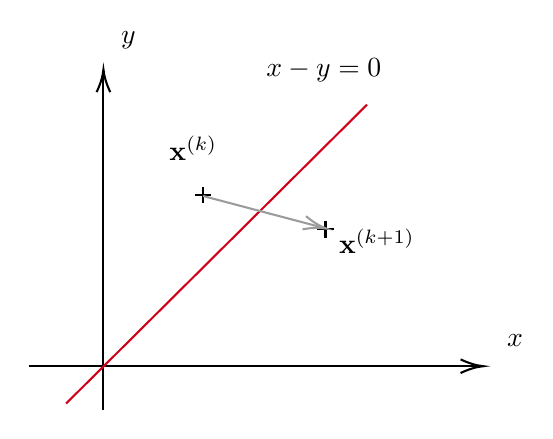
\begin{tikzpicture}[x=0.75pt,y=0.75pt,yscale=-1,xscale=1]
%uncomment if require: \path (0,300); %set diagram left start at 0, and has height of 300

%Straight Lines [id:da29679656074971084] 
\draw    (221,232) -- (432,232) -- (438,232) ;
\draw [shift={(440,232)}, rotate = 180] [color={rgb, 255:red, 0; green, 0; blue, 0 }  ][line width=0.75]    (10.93,-3.29) .. controls (6.95,-1.4) and (3.31,-0.3) .. (0,0) .. controls (3.31,0.3) and (6.95,1.4) .. (10.93,3.29)   ;
%Straight Lines [id:da8887887549358049] 
\draw    (257,253) -- (257,91) ;
\draw [shift={(257,89)}, rotate = 90] [color={rgb, 255:red, 0; green, 0; blue, 0 }  ][line width=0.75]    (10.93,-3.29) .. controls (6.95,-1.4) and (3.31,-0.3) .. (0,0) .. controls (3.31,0.3) and (6.95,1.4) .. (10.93,3.29)   ;
%Straight Lines [id:da36164820457619884] 
\draw [color={rgb, 255:red, 208; green, 2; blue, 27 }  ,draw opacity=1 ]   (239,250) -- (384,106) ;
\draw   (301.04,149.39) -- (308.96,149.39)(305,145.43) -- (305,153.36) ;
\draw   (360.04,166.06) -- (367.96,166.06)(364,162.1) -- (364,170.02) ;
%Straight Lines [id:da4546673743664529] 
\draw [color={rgb, 255:red, 155; green, 155; blue, 155 }  ,draw opacity=1 ]   (305,150) -- (362.4,165.16) ;
\draw [shift={(364.33,165.67)}, rotate = 194.79] [color={rgb, 255:red, 155; green, 155; blue, 155 }  ,draw opacity=1 ][line width=0.75]    (10.93,-3.29) .. controls (6.95,-1.4) and (3.31,-0.3) .. (0,0) .. controls (3.31,0.3) and (6.95,1.4) .. (10.93,3.29)   ;

% Text Node
\draw (334,82.4) node [anchor=north west][inner sep=0.75pt]    {$x-y=0$};
% Text Node
\draw (287.33,119.4) node [anchor=north west][inner sep=0.75pt]    {$\mathbf{x}^{( k)}$};
% Text Node
\draw (369,164.4) node [anchor=north west][inner sep=0.75pt]    {$\mathbf{x}^{( k+1)}$};
% Text Node
\draw (450,215.4) node [anchor=north west][inner sep=0.75pt]    {$x$};
% Text Node
\draw (264,69.4) node [anchor=north west][inner sep=0.75pt]    {$y$};


\end{tikzpicture}

  \caption{距离为0约束}\label{fig:xy0}
\end{figure}

假定当前时间步的位置更新为$\mathbf x^{n} \rightarrow \mathbf x^{n+1}$,由隐式时间积分公式可知,我们认为在时间当前时间步内,所有的单纯形按照匀速直线运动,如下图所示。由于其中穿越了线性流形 $x-y = 0$,即存在时刻 $t \in [0, 1]$,使得$d(t \mathbf x_{n+1} + (1 - t) \mathbf x_{n}) = 0$ ,因此在这一时间步中发生了碰撞,需要进行正确的碰撞处理。


需要指出的是,碰撞处理的实质是避免让几何物体在任意时间发生相交,即距离为 $0$。因此,可以认为在时间积分的过程中存在一不等式约束,许多算法被提出以适应该约束。

%对于三位空间中的网格物体,仅需要考虑如下几类的单纯形之间的碰撞,即可实现几何形体之间的碰撞处理:
%\begin{enumerate}
%  \item 点-三角碰撞
%  \item 边-边碰撞
%\end{enumerate}
%对于维度更低的情况,例如点-边,点-点等碰撞将被纳入上述两类碰撞进行类似的检测和处理。
%Ref:Fast continuous collision detection using deforming nonpenetration filters Tangming.

惩罚函数法是用于碰撞响应的常用算法。其在计算机游戏、动画应用中都有较为广泛的应用。对于空间中的两个几何物体,惩罚函数法试图通过使用类似弹簧的恢复力来惩罚约束违规来避免碰撞的发生,从而实现碰撞处理。例如,考虑\ref{fig:penalty-force-illust}中所示的场景,其中连接了两个刚体的末端。作为惩罚方法的简单说明,我们添加一个原长为$0$的弹簧,用于连接刚体的两端,如下图所示。
\begin{figure}[hbt]
  \centering
  \includegraphics[width=0.5\linewidth]{img/Screenshot 2023-04-23 at 10.32.55.png}
  \caption{惩罚函数法处理碰撞:对于刚体1、2在碰撞点处建立弹簧,用弹簧的力来模拟碰撞的力,从而保证动量守恒。}\label{fig:penalty-force-illust}
\end{figure}

在时间积分时,计算该弹簧的受力,以避免两刚体的碰撞。惩罚函数法也可以不采用弹簧模型,而使用非线性的能量模型来避免需要人为设置的弹簧劲度系数参数。

惩罚函数法使用简单,但其确实存在缺点。例如,对于弹簧劲度系数$k$的设置,过高的的设置会将给系统引入额外的能量,过低的设置则不足以避免碰撞。而且,由于弹簧振动的性质,对于物体之间静止的场景难以用惩罚函数法实现。尽管如此,惩罚函数法仍然是用于处理约束、碰撞的一大类方法。

在数学上,惩罚函数法是在优化问题中处理约束的常用方法。惩罚方法用一系列无约束问题代替约束优化问题,这些问题的解理想地收敛于原始约束问题的解。无约束问题是通过在惩罚约束违规的目标函数中添加一项(称为惩罚项)而形成的。惩罚项在违反约束时较大,在满足约束时较小。惩罚方法依赖于迭代法求解,它从对解的初始猜测开始,然后反复求解一系列无约束问题,惩罚参数不断增加,直到收敛。%Ref Wikipedia

在图形学的碰撞处理中,由于一般的惩罚函数法在极端情况下不能保证没有相交情况,因此2020年 Li 等人提出了基于内点法的增量势能方法(Incremental Potential Contact, IPC)。内点法(也称为障碍函数法或IPM)是解决线性和非线性凸优化问题的一类算法,是惩罚函数法中的一类方法。内点法是一种迭代方法,它从对解的初始猜测开始,然后以越来越高的精度重复求解一系列线性或非线性规划问题,直到收敛。 % Ref: Wikipedia,IPC

增量势能接触(IPC)是一种用于变分求解隐式时间步长新模型和算法。它用于模拟接触变形固体的复杂相互作用。IPC 旨在对真实世界的接触弹性进行有效的时间步长精确和一致的仿真。IPC算法在原先隐式时间积分公式\ref{eq:impl-opt-of}的基础上,加入了距离非零的惩罚函数项 $B(\mathbf x)$
\begin{equation}\label{eq:barrier-func}
  B(\mathbf x) = \sum_{i \in \mathcal C} B(d_i(\mathbf x)), \quad B(d)= \begin{cases}
-(d - \hat d) ^ {2} \log \left(\frac{d}{\hat d}\right) & 0 < d < \hat d\\
0 & \mathrm{otherwise}
\end{cases}
\end{equation}
其中,$\mathcal C$ 表示所有可能的碰撞对,从而优化问题转化为一无约束的优化问题:
\begin{equation}\label{eq:ipc-opt-problem}
  \argmin{\mathbf{x}} E(\mathbf{x}) + B(\mathbf{x})
\end{equation}

在该框架下,碰撞处理转化为使用内点法迭代规避所有可能发生的碰撞,并在将要发生碰撞时,施加足够大的惩罚力。内点法要求每一次迭代更新 $\mathbf{x}^{(k)} \rightarrow \mathbf{x}^{(k+1)}$ 都满足
\begin{equation}
  \forall t \in [0, 1], E((1-t)\mathbf{x}^{(k)} + t \mathbf{x}^{(k+1))} + B((1-t)\mathbf{x}^{(k)} + t \mathbf{x}^{(k+1)}) < \infty
\end{equation}

\begin{algorithm}
  \caption{简化的IPC算法}\label{alg:ipc-sim}
  \begin{algorithmic}[1]
    \Require 当前位置$\mathbf x^{n}$
    \Ensure 积分结果 $\mathbf x^{n+1}$
    \State $\mathbf x^{(0)} \leftarrow \mathbf x^{n}$, $k \leftarrow 0$
    \State $\mathcal C \leftarrow \emptyset$
    \While{$\varepsilon > \varepsilon_0$ and $k < N$}
      \State $\mathbf d \leftarrow - H^{-1}\nabla_{\mathbf x}(E(\mathbf x) + B(\mathbf x))$
      \State 对 $\mathbf d$ 执行线搜索,确定系数$\alpha$
      \State $\mathbf x'\leftarrow \mathbf x + \alpha \mathbf d$
      \State 检查$\mathbf x^{(k)} \rightarrow x'$碰撞情况,最小碰撞时间为 $ 0 < \alpha' \le 1$,更新 $\mathcal C$
      \State $\mathbf x^{(k+1)} \leftarrow \mathbf x^{(k)} + \alpha' \mathbf d$
      \State $k\leftarrow k + 1$
    \EndWhile
    \State \Return $\mathbf x^{(k)}$
  \end{algorithmic}
\end{algorithm}


一个简单的IPC算法如\ref{alg:ipc-sim}所示。与原先论文的算法相比,该算法提炼了IPC的核心思想,即内点法:算法\ref{alg:ipc-sim}的第7、8步保证了每一次位置更新前都检查其更新轨迹不发生相交,从而处理了所有可能的碰撞。其中,算法的第4步中使用了优化函数的Hessian矩阵$H$获取更好的迭代方向,第5步使用线搜索,计算了一个可以使得目标函数充分下降的迭代步长。由于线搜索后执行了碰撞检测,并且该方向是一个下降方向,步长保证无碰撞发生,因此IPC确保了时间积分能够正确收敛到能量函数最小的位置,并且该时间步不发生穿透。

该算法的缺点在于,即使 $E$ 具有一个固定的 Hessian 矩阵,例如弹簧质点模型,由于 $B$ 的Hessian阵在每一个时间步都有可能发生变化,其也无法应用稀疏 Cholesky 分解等预计算加速方法进行快速矩阵计算。这对于复杂场景、复杂对象的解算是十分不利。

总而言之,对于碰撞处理问题,惩罚函数法是一类常用的解决方案。近年来,由于IPC算法的提出,基于内点法的碰撞处理又成为了研究焦点。对于流固耦合算法而言,可以转化为流体粒子与固体之间的完全非弹性碰撞,应用相关算法得以解决。本文的主要工作将从该重要的观察出发,进行基于惩罚函数法实现的流固耦合算法研究。

